\section{Design and Manufacturing I}

\begin{center}
    Notes from \textbf{MECHENG 250: Design and Manufacturing I}
    
    Taken at University of Michigan, Winter 2025
\end{center}

\subsection{Product Design}
In general, a product undergoes various phases of design: \begin{enumerate}
    \item Specifying \textit{functional requirements}, i.e. design-neutral, measurable goals which the product must accomplish
    \item Product \textit{ideation}, including research in existing solutions and generation of initial designs
    \item \textit{Analysis}, using first-principles models
    \item \textit{Performance evaluation}, where empirical data is analyzed by some means, i.e. by a regression model
\end{enumerate} These steps may repeat any number of times until a design is satisfactory.

A simplified \textit{first principles model} is often useful for evaluating feasibility of a design. A first-principles model typically involves drawing a free-body diagram, then using Newton's and Euler's equations to evaluate forces and moments acting on the body. Such analysis often gives a desired output as a function of \textit{design variables}--properties which can be changed to influence the ability of the product to perform, such as length, material, and so on.

An \textit{empirical model} is produced by extrapolating from real-world data, typically through some kind of regression model which relates a desired output to a variable, tested input. A regression model works by minimizing the square of the error between extrapolated values and observed values.

\newpage

\subsection{Machine Elements}

\textbf{Transmissions}

A transmission is a system which transfers power. Common transmissions involves \textit{gears}, \textit{belts}, or \textit{chains}. There are various tradeoffs between these components:
\begin{enumerate}
    \item[] \textbf{Gears}. Gears come in many forms and essentially transfer rotational motion through meshing teeth.
    \item[] \textbf{Belts}. Belts are less expensive than gears, but require a tensioner in order to prevent slipping.
    \item[] \textbf{Chains}. Chains are connected to two sprockets. Chains are often less expensive than gears and, unlike belts, do not require a tensioner.
\end{enumerate} These transmission systems are mathematically identical, and the following relationships hold (in magnitude): \[\frac{\omega_2}{\omega_1} = \frac{T_1}{T_2} = \frac{d_1}{d_2} = \frac{N_1}{N_2}\]

For two gears to mesh, the \textit{diametral pitch} $P$ and pressure angle. Diametral pitch is given by \[P = \frac{N}{d}\]

A \textit{gear train} is a system consisting of several gears. The \textit{gear speed ratio} $e$ for a gear train is given by \[e = \frac{\omega_\text{output}}{\omega_\text{input}} = -\frac{d_1}{d_2} = \underbrace{\frac{n_\text{output}}{n_\text{input}}}_\text{speed (RPM)}\] From a conservation of energy, torque is given by \[T_2 = \eta\frac{T_1}{e} = \eta T_1 \frac{N_2}{N_1}\] where $\eta$ is the gear efficiency, where $\eta$ is typically between $0.9$ and $0.95$ \textit{per contact on a gear train}. 

\textbf{Electric Motors}

A \textit{motor} is a common device which converts electrical power to mechanical power. A motor is defined by a no-load speed $n_0$ (with no output torque) and stall torque $T_s$ (with zero speed). A \textit{torque-speed curve} is an approximately linear relationship between output torque $T$ and speed $n$, where \[T = T_s - kn\] A torque-speed curve has slope $1/k$ and shows speed $n$ as a function of torque $T$. If a motor is too weak, it is often useful to use a gear train to increase maximum effective torque at the expense of speed, according to the relationship \[\frac{T_{s2}}{\gamma T_{s1}} = \frac{n_{01}}{n_{02}} = M\] where $\gamma$ is the efficiency of the geartrain and $M$ is the gear ration M:1 for a gearbox. Alternatively, increasing the voltage of a gearbox shifts the torque-speed curve up, according to the relationship: \[\frac{T_{s2}}{T_{s1}} = \frac{n_{02}}{n_{01}} = \frac{V_2}{V_1}\]

\newpage

\textbf{Springs}

A \textit{spring} is a common device which is meant to apply a controlled force or torque and/or store potential energy. Linear springs are of potential interest, where the number of turns $N_t$ on the spring is given by \[N_t = \frac{L_s}{d}\] where $L_s$ is spring length when fully compressed and $d$ is the diameter of the coil wire. There are two primary types of linear springs:
\begin{enumerate}
    \item[] \textbf{Extension Spring}. Number of active coils $N_a = N_t$. Contains an initial preload $F_\text{initial}$, so $F_\text{s,ext} = F_\text{initial} + k\delta$.
    \item[] \textbf{Compression Spring}. Number of active coils $N_a = N_t - 2$ because the ends are inactive. Compressive force given by $F_\text{s,ext} = k\delta$.
\end{enumerate}

If the mean coil diameter $D_m$ and the material's shear modulus $G$ is known, the spring constant $k$ may be calculated as follows: \[k = \frac{F}{\delta} = \frac{Gd^4}{8D_m^3N_a} = \frac{Gd}{8C^3N_a}\] where $C$ is the \textit{spring index}, defined by $C = D_m/d$.

\textbf{Lead Screws}

A \textit{lead screw} is a screw which rotates, causing a nut to translate. These systems are simple, but low efficiency and typically quite slow. To raise a load of weight $F$ given a lead screw with pitch diameter $D_p$, screw lead $l$, pitch $p$ (distance between two threads), and coefficient of friction $\mu$, the torque to raise and lower a load respectively is given by \[T_\text{raise} = \frac{FD_p}{2}\left(\frac{l+\mu\pi D_p}{\pi D_p - \mu l}\right),\hspace{0.25in} T_\text{lower} = \frac{FD_p}{2}\left(\frac{\mu \pi D_p - l}{\pi D_p + \mu l}\right)\]

\textbf{Mechanisms}

A \textit{mechanism} is any device which transfers motion and/or force from an input to an output. A \textit{linkage} is a specific type of mechanism which consists of links connected at joints. A group of linkages forms a \textit{kinematic chain}, which may be \textit{open} (free at one end) or \textit{closed} (fixed at both ends). 

A \textit{four-bar linkage} is a common type of linkage consisting of four links and four joints, where a single motor may be used to control the linkage. Given a four-bar linkage with shortest link of length $s$, longest link of length $l$, and the other links of length $p,q$, by \textbf{Grashof's Criterion}, the linkage may complete a 360-degree rotation relative to the ground if and only \[s+l < p+q\]

%\newpage

\subsection{Dimensioning and Tolerancing}

Any two of the same part will have differing dimensions, introducted through variation in the manufacturing process (tool wear, machine precision, measurement inaccuracy, etc). \textit{Tolerance} is the total size variation allowed in a part, given by \[\text{tolerance} = \text{upper limit}-\text{lower limit}\] The \textbf{basic size} of a part is the size around which tolerances are calculated. The \textbf{maximum material condition (MMC)} is the size of the part where it has the most material (i.e. smallest hole or largest shaft), and \textbf{least material condition (LMC)} is the size of the part where it has the least material (i.e. largest hole or smallest shaft). Measurement of MMC and LMC are useful for evaluating whether components can fit together at the limits of tolerance. For example, for a shaft and hole, \[\text{max clearance}=\text{LMC}_\text{hole}-\text{LMC}_\text{shaft},\hspace{0.2in}\text{min clearance} = \text{MMC}_\text{hole}-\text{MMC}_\text{shaft}\]

Standard dimensioning and tolerancing is often insufficient for ensuring a part will function. \textit{Geometric Dimensioning and Tolerancing} (GD\&T) allows parts to be more accurately defined, often with larger tolerances and fewer opportunities for misinterpretation. A \textit{feature control frame} is used to place a tolerance on a geometric feature with respect to a datum point on a part, as shown:

\begin{center}
    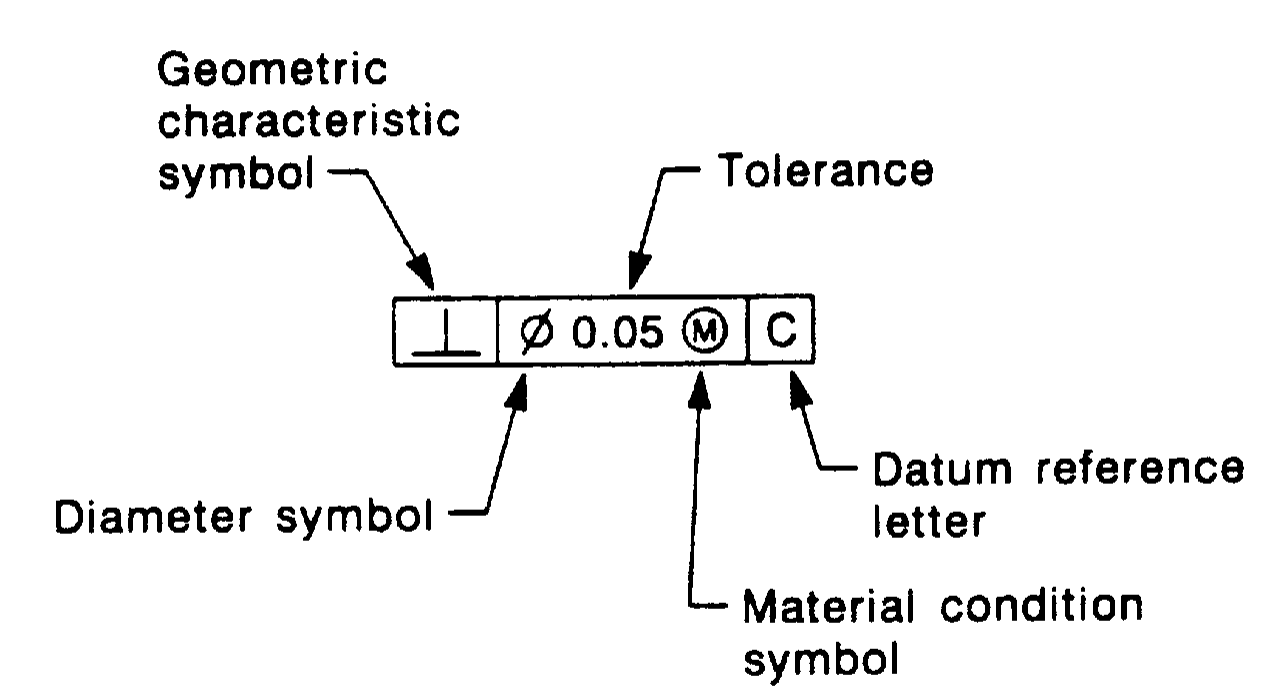
\includegraphics[scale=0.3]{Images/x50_gd&t.png}
\end{center}

where M and L refer to maximum and least material conditions, respectively. Characteristics may be any of the following:

\begin{center}
    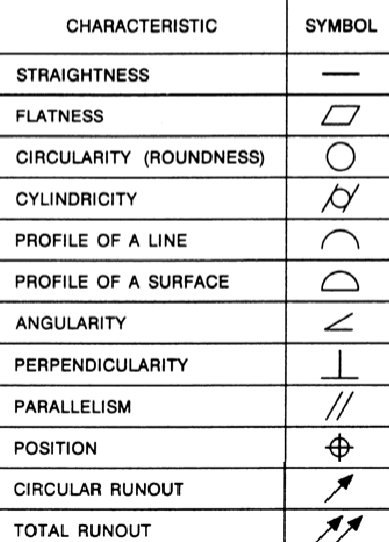
\includegraphics[scale=0.6]{Images/x50_gd&t2.png}
\end{center}

\subsection{Manufacturing Systems}

\textbf{Discrete Manufacturing}

\textit{Discrete manufacturing} refers to the production of distinct items (as opposed to \textit{process manufacturing}, where production is by weight, i.e. chemical or pharmaceutical production). Discrete manufacturing systems can generally be analyzed as a production line, consisting of a series of separate manufacturing stations.

The production rate of an entire line is limited to the production rate of the slowest machine, where the slowest machine is the \textit{bottleneck}. Optimizing the flow rate of a production line therefore involves optimizing the output of the bottleneck. Common ways to improve a process bottleneck include: \begin{enumerate}
    \item Add another bottleneck process in parallel, thus increasing the effective production rate
    \item Place a \textit{buffer} station (accumulating parts from a previous station) before the bottleneck to prevent the bottleneck being \textit{starved}.
\end{enumerate}

Discrete manufacturing occurring over a long period of time may be approximated as a steady-state flow, with constant flow rate $\lambda$ parts per hour. \textbf{Little's Law} simply relates the production rate and the time of production $W$: \[L = \lambda W\] Importantly, Little's Law applies to both a single process and a group of processes (i.e. an entire factory). Therefore, $L$ may be either the number of units in a system or the number of manufacturing stations in a factory, depending on the units of the variable $\lambda$.

\textbf{Takt time} is a measure of the average time between production of units, given by \[\text{takt time} = \frac{\text{production time}}{\text{production quantity}}\] If $1/\lambda > \text{takt time}$, then the production system is too slow and/or the production numbers are unfeasible in the given time.

\textbf{Process Capability}

A \textit{process capability index} is a standard way to measure the variability of a process output within a specification or tolerance. Given an \textit{upper specification limit} USL and a \textit{lower specification limit} LSL, the process capability index $C_p$ is defined by \[C_p = \frac{\text{USL}-\text{LSL}}{6\sigma}\] where $\sigma$ is the standard deviation of measurements on output parts. $C_p$ should ideally be as large as possible, with $C_p>1.33$ being the typical industry-standard minimum. $C_{pk}$ measures both the accuracy and the precision by comparing to the mean value, where $C_{pk}$ is defined by \[C_{pk} = \min \left\{\frac{\text{USL}-\mu}{3\sigma},\frac{\mu-\text{LSL}}{3\sigma}\right\}\] $C_{pk}$ is generally smaller than (or sometimes equal to) $C_p$ and should also be maximized.

\textbf{Manufacturing Cost Modeling}

Total costs involved in the production of $n$ parts of mass $m$ are given by \[C_\text{total} = C_\text{material} + C_\text{capital} + C_\text{energy} + C_\text{overhead}\] Many processes are only viable given large batch size, effectively reducing per-part capital costs.

Whether an investment is likely to be profitable is determined by the related quantities \textit{net present value} (NPV) and \textit{internal rate of return} (IRR). Given an initial investment $C_\text{init}$, cash flow $C_t$ in year $t$, and discount rate (annual return that could be earned with a similar investment, typically between 5\% and 15\%) $i$, the net present value of an investment is computed as \[\text{NPV} = \sum_{t=1}^T\underbrace{\left(\frac{C_t}{(1+i)^t}\right)}_\text{Yearly NPV} - \underbrace{C_\text{init}}\] Similarly, the internal rate of return is the value for which $\text{NPV}=0$, or the solution to \[\sum_{t=0}^T \left(\frac{C_t}{(1+\text{IRR})^t}\right) - C_\text{init} = 0\] If $\text{IRR}<i$, an investment is a bad investment as it does not meet the minimum rate of return a firm could achieve with a similar investment. A higher IRR indicates a more desirable investment, and the best investment among a series of options is that with the highest IRR.

\subsection{Manufacturing Processes}

Manufacturing most fundamentally involves bringing stock material to a desired shape. Each manufacturing process has specific capabilities and associated processing times, making a process more or less feasible depending on the material properties, desired geometry, and the scale of production. 

\textbf{Subtractive Processes}

Subtractive processes involve removing material from a stock piece. Common examples include:
\begin{enumerate}
    \item[] \textbf{Blanking}, a process by which sheet-metal components are produced by shearing. This process is suitable for mass production because of its low processing time and the recyclability of leftover material "skeleton".
    \item[] \textbf{Machining}, where the five basic machining processes are \textit{turning} (on a lathe), \textit{drilling}, \textit{milling}, \textit{grinding}, and \textit{sawing}.
    \item[] \textbf{CNC Processes}, including water jetting, laser cutting, CNC milling, CNC lathing, and other automated processes. CNC machines are programmed with G-Code and generally allow more complex geometries to be produced (in particular with CNC mills and CNC lathes).
\end{enumerate}
Machining processes are relatively slow compared to other methods, and are therefore not suitable for mass manufacturing (i.e. $>$100,000 parts). As an example, for a lathe operation with feed rate $f$ inches/rev, spindle speed $N$ revs/min, initial diameter $D_0$ and a depth of removal $d$, the material removal rate is given by \[\text{material removal rate} = \underbrace{\pi D_0 N}_{v} d f\] where $v$ is the \textit{cutting speed}, the tangential speed of the workpiece. The machining time is then given by \[T_m = \frac{L}{Nf}\]

\textbf{Metal Forming}

Because machining is relatively slow, parts are generally brought near their final shape so that machining becomes a finishing process, rather than a shaping process. The processes here are \textit{bulk deformation processes}, which plastically deform a material, causing \textit{work hardening} and producing a tougher final part: \begin{enumerate}
    \item[] \textbf{Extrusion}. Involves forcing a metal through a die to form a long shape. Metals may be extruded \textit{hot} (aluminum, copper, magnesium) or \textit{cold} (aluminum or steel, with steel requiring high forces).
    \item[] \textbf{Forging}. Produces a part near net shape of very high strength. Types include \textit{open die forging} (suitable for large parts, generally requiring lots of machining) and \textit{closed die forging} (suitable for producing smaller parts near net shape, where only the excess "flash" which squeezes out of the mold must be machined away).
\end{enumerate}

The forces involved in forging can be quite large. The required forces can be evaluated by considering first the necessary deformation, then the strain in the material, then the stress in the material, and finally the surface area of the part.

Strain of work is given by \[\epsilon = \ln \frac{h_0}{h}\] where $h_0$ is the initial height of the stock and $h$ is the final height. The stress is then given by \[Y_f = K\epsilon ^n\] where $K$ is the strength coefficient and $n$ is the strain hardening exponent, both of which are material properties. Finally, the compressive force is found by \[F = K_f Y_f A\] where \[K_f = 1 + \frac{.4\mu D}{h} \text{ (shape factor)}\] $K_f$ is a function of part height and diameter, and also friction between the part and the die. Shape factor $K_f$ is not related the strength coefficient $K$.

There are different metal forming operations available for forming sheet metal parts: \begin{enumerate}
    \item[] \textbf{Simple Bending}. Involves bending straight lines into a sheet metal part using a punch and die. Both cheaper and slower than stamping operations.
    \item[] \textbf{Sheet Metal Stamping}. Involves pressing a sheet metal part between a die and a punch to form a desired shape. Often used in mass production because the process is relatively fast and maintains sheet thickness.
    \item[] \textbf{Sheet Metal Drawing}. Essentially the same as stamping, but with a specialized (more expensive) die allowing part to be drawn to a depth larger than the punch diameter.
\end{enumerate}

\textbf{Additive Manufacturing}

Additive manufacturing processes are varied and involve forming a part from feedstock, rather than forming or removing from existing stock. There are seven categories of additive manufacturing process:

\begin{center}
    \begin{tabular}{ | m{2in} | m{2in} | m{2in} | }
    \hline
    Process & Material Used & Tool Used\\
    \hline
    Material Jetting & Melted Plastic & Laser or Multi-Nozzle Print Head\\
    \hline
    Vat Photopolymerization / Stereolithography (SLA) & Melted Plastic & Laser\\
    \hline
    Material Extrusion & Melted Plastic & Single-Nozzle Print Head\\
    \hline
    Sheet Lamination & Material Sheets & Solid-State Welding or Adhesive\\
    \hline
    Directed Energy Deposition & Powdered Metal & Laser \\
    \hline
    Powder Bed Fusion & Plastic Powder (SLS) or Metal Powder (SLM/DMLS) & Laser\\
    \hline
    Binder Jetting & Powdered Metal & Multi-Nozzle Print Head, then Solid State Welding\\
    \hline
    \end{tabular}
\end{center}

\textbf{Liquid to Shape}.

As opposed to other metal forming processes, metals can also be \textit{cast} into a nearly complete shape. This is accomplished by pouring a molten metal into some form of mold; the hardened metal then takes the desired shape. This process generally requires some amount of machining to process the part, particularly for threads and smooth surfaces, both of which casting is incapable of producing. There are two types of casting: \begin{enumerate}
    \item[] \textbf{Die Casting}. Metal is forced into a permanent die cavity under pressure. Allows for high production rate (suitable for mass manufacturing) and good tolerances and surface finish. Can occur in a \textit{hot chamber} (where low melting point metals, i.e. zinc or magnesium, are under high pressure until they solidify in the mold) or in a \textit{cold chamber} (where metal is melted in a separate furnace and driven into the die). 
    \item[] \textbf{Sand Casting}. Most common casting process, involving a mold made of sand which is broken after the part solidifies. Produces a rough surface finish and has low upfront cost, but is also a slower process as molds are not reused.
\end{enumerate}

A mold used in sand casting consists of a \textit{cope} (top half) and \textit{drag} (bottom half), and often a \textit{core} which produces the internal surfaces on a cast part. The core is supported by \textit{chaplets} both above and below, which are placed below to support the core weight and above to counteract bouyant forces from the molten metal. For core of density $\rho_c$ and volume $V_c$ and molten metal of density $\rho_m$, the forces acting on the core are \[\underbrace{F_b = (\rho_m - \rho_c)V_cg}_\text{bouyant force},\hspace{0.5in}\underbrace{W=\rho_cV_cg}_\text{weight}\] If a chaplet is able to support $F_\text{chap}$, then the number of chaplets necessary is given by \[N_\text{above} = \left\lceil\frac{F_b}{F_\text{chap}}\right\rceil\] Then, enough chaplets must be placed below to support the weight of both the core and the chaplets above. Thus, the number of chaplets required below is \[N_\text{below} = \left\lceil\frac{W +N_\text{above}\cdot W_\text{chap}}{F_\text{chap}}\right\rceil\]

\newpage

Even more diverse processes exist for forming liquid plastic:
\begin{enumerate}
    \item[] \textbf{Injection Molding}. Produces open shapes by forcing high-pressure liquid plastic into a closed mold. Plastic is subject to shrinkage as it cools.
    \item[] \textbf{Blow Molding}. Produces thin, bottle-like shapes with small openings by "blowing" heated plastic to walls of a closed mold.
    \item[] \textbf{Rotational Molding}. Produces thin-walled, seamless, hollow shapes by rotating a mold, forcing liquid plastic to conform to the mold shape.
    \item[] \textbf{Thermoforming}. Produces flat, thin-walled shapes by "sucking" heated plastic sheet onto an open mold.
\end{enumerate}

Parts created in injection molding are particularly vulnerable to shrinkage as they cool within the mold. If a cavity has dimension $D_c$ and a plastic has a shrinkage value $S$ (typically in mm/mm or inch/inch, i.e. unitless), then the dimension of the molded part is given by \[D_c = \frac{D_p}{1-S}\]